\documentclass[a4paper, 11pt, twoside]{report}

    % preambule {{{

    % TODOS
    \usepackage[colorinlistoftodos]{todonotes}

	\usepackage[utf8]{inputenc}
	\usepackage[T1]{fontenc}
    \usepackage[frenchb]{babel}
    \usepackage{textcomp}
	\usepackage[top=3cm,left=3cm,right=3cm,bottom=3cm]{geometry}
    \usepackage{lmodern}
    \usepackage{sectsty}
    \usepackage{nicefrac}
	\usepackage{graphicx}
    \usepackage{lastpage}
    \usepackage{fancyhdr}
    \usepackage{amsmath}
    \usepackage{amssymb}
    \usepackage{amsfonts}
    \usepackage{capt-of}
    \usepackage{caption}
    \usepackage{subcaption}
    \usepackage{wrapfig}
    \usepackage{bm} % bold math
    \usepackage{tikz}

    \usepackage{fancyvrb} % pour forcer les verbatim sur une seule page
    \usepackage{url}

	\title{Couplage des méthodes FEM et DGM}
	\author{Mathieu \textsc{Gaborit} \hfill Encadrant : Olivier \textsc{Dazel}}
	\date{M1 Acoustique
    \vskip 2mm
    Année universitaire 2014-2015}

	\makeatletter
	\def\thetitle{\@title}
	\def\theauthor{\@author}
	\def\thedate{\@date}
	\makeatother

    \sectionfont{
    \sectionrule{0pt}{0pt}{-5pt}{0.4pt}
    }

    % interligne
    \renewcommand{\baselinestretch}{1.1}

    \setcounter{secnumdepth}{5}
    \setcounter{tocdepth}{3}
    \addto\captionsfrench{\renewcommand{\chaptername}{Partie}}
    \renewcommand{\thechapter}{\arabic{chapter}}
    \renewcommand{\thesection}{\Roman{section}.}
    \renewcommand{\thesubsection}{\Alph{subsection})}
    \renewcommand{\thesubsubsection}{\arabic{subsubsection}.}
	\renewcommand{\theparagraph}{}


    \pagestyle{fancy}

    \fancypagestyle{plain}{%
        \fancyhf{} % clear all header and footer fields
        \renewcommand{\headrulewidth}{0pt}
        \renewcommand{\footrulewidth}{0pt}
    }

    \fancypagestyle{toc}{%
        \fancyhf{} % clear all header and footer fields
        \fancyfoot[L]{\textsc{Gaborit}}
        \fancyfoot[C]{}
		\fancyfoot[R]{\thepage}
        \renewcommand{\headrulewidth}{0pt}
        \renewcommand{\footrulewidth}{.4pt}
    }
	\AtBeginDocument{\addtocontents{toc}{\protect\thispagestyle{toc}}} 


    \renewcommand{\headrulewidth}{0pt}
    \renewcommand{\footrulewidth}{.4pt}
    \lhead{}
    \chead{}
    \rhead{}
    \lfoot{\textsc{Gaborit}}
    \cfoot{}
    \rfoot{\thepage/\pageref{LastPage}}


	\newcommand\DP{\delta p}
\newcommand\dd{\mathrm{d}}
\newcommand\ul{\underline}
\newcommand\uul[1]{\underline{\underline{#1}}}
\newcommand\ult[1]{\tilde{\underline{#1}}}
\newcommand\uult[1]{\tilde{\underline{\underline{#1}}}}

\newcommand\matlab{MATLab\textsuperscript{\textregistered}}
\renewcommand\equiv{\Leftrightarrow}
\newcommand\diag{\mathrm{diag}}
\renewcommand{\phi}\varphi

\renewcommand\H[1]{\tilde{h_{#1}}}
\newcommand\Hp[1]{\tilde{h'_{#1}}}

\renewcommand\GU{\mathbb{U}}
\renewcommand\GV{\mathbb{V}}
 % typesetting commands (part. for math)
    % }}}

\begin{document}


% page de titre [PAS TOUCHE] {{{1
\begin{titlepage}

% logo Univ
\begin{flushright}

\includegraphics[width=4cm]{logo.png}
\end{flushright}


\vskip 6cm

% Titre
\begin{flushleft}
\huge{\textbf{\thetitle}}
\vskip .5cm
\hrule height 3pt
\vskip .5cm
\hfill\huge{\textbf{Rapport de projet}}
\end{flushleft}

\vfill

\begin{center}
\Large{
\thedate
}
\end{center}

\vskip 1cm
\hrule height .5pt
\vskip .5cm

\begin{flushleft}
\theauthor
\end{flushleft}

\end{titlepage}


\newpage\thispagestyle{empty}\null\newpage

\pagenumbering{roman}
\rfoot{\thepage}
\setcounter{page}{1}
\section*{Remerciements}

Parce que ce projet a généré beaucoup de questions et parce qu'il a été un encadrant toujours disponible pour y répondre, je tiens
à remercier Olivier Dazel. Je tiens aussi à remercier Gwenaël Gabard qui a pris un peu de temps pour discuter du
projet lors de son passage au Mans.

Ce travail est axé sur les méthodes numériques et assez peu de choses auraient été faisables sans les contributeurs à
GNU/Octave~\cite{octave}, mais aussi à IPython~\cite{ipython} (nouvellement Jupyter\footnote{\url{http://jupyter.org}}),
merci à eux.

De même, je remercie du fond du coeur tous les contributeurs aux projets de la Wikimedia
Foundation\footnote{\url{http://wikimedia.org}} pour le travail impressionnant qu'ils réalisent chaque jour et la masse
de connaissances qu'ils mettent à disposition.

Enfin, je tiens à remercier tous les relecteurs qui ont grandement amélioré la qualité de ce rapport.


\section*{Abstract}

As comptuation power and problems complexity increase, designing efficient numerical methods is a major challenge.

Some, among the large amount of available methods, have been known and used for years, but each is often limited to
certain types of problems. The key idea behind the present work is to prepare coupling between Finite Elements
Method (FEM) and Discontinuous Galerkin Method (DGM).

As FEM is particularly well-suited for small and detailled configurations and plane waves based DGM allows efficient modelling of
propagation in large cavities without too much details, coupling of both would lead to great improvements in
numerical computation of propagation in complex medium.

This document uses classical FEM formulation and the plane waves based DGM formulation recently proposed by
Gabard \textit{et al.}~\cite{Gabard15,Gabard11} as a basis. Both methods are succintly introduced and a coupling possibility
based on the rewriting of FEM boundary conditions using a DGM-compatible approach is then studied.

As this modification has a non-negligible impact on convergence of the method, a new interpolation functions basis
using Hermite splines is proposed.

The convergence rate and overall accuracy of the final method (based on rewritten boundary conditions and Hermite
splines) are finally shown to be better than those of the method based on classical FEM boundary conditions and
quadratic elements.

\paragraph{Keywords:} Helmholtz; finite elements; discontinuous Galerkin; coupling; convergence


\newpage
% sommaire [PAS TOUCHE] {{{1
\renewcommand{\contentsname}{Sommaire
\vskip .5cm
\hrule height .5pt}
\tableofcontents
\newpage
\pagestyle{fancy}


% Chapitres {{{1
\rfoot{\thepage/\pageref{LastPage}}
\pagenumbering{arabic}
\setcounter{page}{1}
\section*{Introduction}

À mesure que la puissance des ordinateurs explose et que la science avance, les méthodes numériques représentent un
enjeu de plus en plus important. Aujourd'hui, la complexité des problèmes engagés est telle que les solutions
analytiques sont parfois impossibles à déterminer.

Après des années de recherche, de plus en plus de méthodes ont vu le jour pour pallier ce manque et ce dans quasiment
tous les domaines scientifiques. Depuis les méthodes spectrales jusqu'aux algorithmes évolutifs, la science moderne est
avide de méthodes d'approximation et d'automatisation efficaces et celles-ci sont en constant développement. De plus,
la comparaison entre les différentes méthodes présente un intérêt majeur pour réaliser ensuite des choix
avisés~\cite{Gabard11}.

Connues depuis des décennies, les méthodes visant à discrétiser le milieu de travail ou le temps sont un des cas
d'étude classiques, la méthode des éléments finis (FEM) en fait partie. Pourquoi ne pas résoudre plein de petits problèmes
simples plutôt qu'un unique problème complexe ? La discrétisation des variables n'est toutefois pas l'unique solution
envisageable...

Mises au point au début du XX\textsuperscript{ème} siècle, les méthodes de Galerkin suivent, elles, un autre chemin vers le
problème discret : en plus d'une discrétisation en espace, elles proposent aussi de chercher la solution du problème
sous la forme d'une somme de fonctions plus simples. Améliorées dans les années 1970 en méthodes de Galerkin
discontinues (DGM), elles permettent alors la résolution d'équations aux dérivées partielles (EDP).

Ces deux méthodes sont classiques et bien connues des chercheurs, elles ont toutefois leurs spécificités quant aux
problèmes qu'elles permettent de résoudre de manière consistante.

\bigskip

L'objectif de ce projet est de s'intéresser au couplage entre la FEM et la DGM en se basant sur la ré-écriture des
conditions limites de la FEM.

Dans un premier temps, les deux méthodes sont succintement présentées et un exemple d'utilisation est proposé.
Dans un second temps, la possibilité de ré-écriture des conditions aux limites du domaine FEM est analysée et une
nouvelle formulation basée sur le parallèlisme avec les caractéristiques utilisées dans la DGM avec ondes planes est
proposée. Une réflexion sur la convergence de cette méthode modifiée amène ensuite à considérer la dernière partie de ce
rapport. Afin de rendre la méthode proposée réellement intéressante, une nouvelle base de fonctions d'interpolation pour
les champs FEM est introduite et son influence sur la convergence est analysée.





\part{Méthode des Éléments finis}
\label{part:fem}
\newpage\thispagestyle{empty}\null\newpage
\addtocounter{page}{-2}
\setcounter{section}{0}

% TODO intro galerkin

\section{Généralités}

Soit un milieu de propagation où sont valable les équations suivantes :

\begin{eqnarray}
    \left\{\begin{array}{l}
        j\omega\rho v = -\nabla p\\
        p = -\rho c^2 \nabla u
    \end{array}\right.
    & \Leftrightarrow &
    \left\{\begin{array}{l}
        j\omega\rho v = -\nabla p\\
        j\omega p = -\rho c^2 \nabla v
    \end{array}\right.
    \notag\\ & \Leftrightarrow &
    j\omega \begin{Bmatrix}v\\p\end{Bmatrix} + 
    \begin{bmatrix}
        0 & \nicefrac{1}{\rho}\\
        \rho c^2 & 0
    \end{bmatrix}
    \nabla \begin{Bmatrix}v\\p\end{Bmatrix} = 0
    \notag\\ & \Leftrightarrow &
        \left(j\omega + \uul{A}\frac{\partial}{\partial x}\right) \ul{u} = 0 \label{dgm:eq_u}
\end{eqnarray}

L'idée est alors de découpler les équations précédentes en diagonalisant $\uul{A}$, il vient :

\begin{equation*}
    \uul{A} = \uul{P\Lambda Q} \quad,\quad \uul{P} = \uul{Q}^{-1}
\end{equation*}

En posant

\begin{equation}
    \ul{\tilde{u}} = \begin{Bmatrix}\tilde{u}^+\\\tilde{u}^-\end{Bmatrix} = \ul{Q}\ul{u}\label{dgm:utilde}
\end{equation}
l'équation~\eqref{dgm:eq_u} devient :

\begin{equation*}
    j\omega \ul{\tilde{u}} + \uul{\Lambda}\nabla\ul{\tilde{u}} = 0
\end{equation*}

En isolant les valeurs positives et négatives de $\uul{\Lambda}$  (notées $\Lambda^{+,-}$) ainsi que les vecteurs
associés $\ul{P}^{+,-}$ et $\ul{Q}^{+,-}$, il est possible d'écrire :

\begin{equation}
    \left\{\begin{array}{l}
        \tilde{u}^+ = \ul{Q}^+\ul{u}\\
        \tilde{u}^- = \ul{Q}^-\ul{u}
    \end{array}\right. \Leftrightarrow
    \ul{u} = \ul{P}^+\tilde{u} + \ul{P}^-\tilde{u} \label{dgm:sep_u}
\end{equation}


\paragraph{Formulation variationnelle}

En utilisant la formulation variationnelle et une intégration par parties, il vient :

\begin{equation}
    \begin{array}{c}
    \int_\Omega \ul{v}^T\left(j\omega + \uul{F}\nabla\right)\ul{u}\dd\Omega = 0 \quad,\quad \forall\ul{v}\\
    -\left(\int_\Omega j\omega v + \uul{A}^T\nabla\ul{v}\right)^Tu\dd\Omega +
        \int_{\partial\Omega}\ul{v}^T\uul{A}\ul{u}\dd\Gamma = 0 \quad,\quad \forall\ul{v}
    \end{array}
    \label{dgm:post_ipp}
\end{equation}

\paragraph{Nota Bene} Le symbole $\cdot^T$ représente une transposition Hermitienne.

L'objectif est alors de choisir le champ de test $\ul{v}$ permettant d'annuler l'intégrale sur $\Omega$ :

\begin{equation}
    \left(j\omega + \uul{A}^T\nabla\right)\ul{v} = 0 \label{dgm:eq_v}
\end{equation}

De toute l'équation~\eqref{dgm:post_ipp}, il reste alors :

\begin{equation}
    \int_{\partial\Omega}\ul{v}^T\uul{A}\ul{u}\dd\Gamma = 0 \quad,\quad \forall\ul{v}\label{dgm:to_solve}
\end{equation}


\section{Fonctions d'interpolation classiques}

La précision et l'efficacité de la méthode des éléments finis repose grandement sur le choix judicieux des fonctions de
forme $\phi$.

Communément, le choix, pour des problèmes en traction/compression, se fait entre des fonctions linéaires et
quadratiques.

Il est nécessaire, lors de la comparaison de ces deux alternatives, de prendre en compte non pas le nombre d'éléments
mais bien le nombre de degrés de liberté\footnote{Points où sont calculées les valeurs des champs utilisées ensuite pour
l'interpolation.}. En effet, le concept derrière l'interpolation avec des polynômes est toujours le même : pour un
polynôme de degré $N$, il faut $N+1$ point.

\subsection{Éléments Linéaires}

La première interpolation possible utilise des fonctions affines. L'idée est alors d'écrire :

$$p = p_1\phi_1(x) + p_2\phi_2(x)$$

Avec $p_{1,2}$ les valeurs du champ à chaque extrémité $x_{1,2}$ et $\phi_{1,2}$ nulles en $x_{2,1}$ et égales à l'unité
en $x_{1,2}$. Ainsi, les deux fonctions ont le profil présenté en figure~\ref{fig:FEM:lin_shape_fun}.

\begin{figure}[!ht]
	\centering
	\begin{tikzpicture}
	\def\h{2};

	% PHI 1
	\draw[thick] plot [domain=0:\h] (\x,{1-\x/\h});
	\draw[->] (-.3,0) -- (\h+.5,0);
	\draw[->] (0,-.3) -- (0,1.5);
	\draw[fill=red] (0,1) circle (.05);
	\draw[fill=red] (\h,0) circle (.05);
	\draw (-.1,1) node[left] {$1$} --++(.2,0);
	\draw (\h,-.1) node[below] {$h$} --++(0,.2);
	\draw (\h*.5,-.5) node {$\phi_1$};

	% PHI 2
	\begin{scope}[shift={(\h+2,0)}]
		\draw[thick] plot [domain=0:\h] (\x,{\x/\h});
		\draw[->] (-.3,0) -- (\h+.5,0);
		\draw[->] (0,-.3) -- (0,1.5);
		\draw[fill=red] (0,0) circle (.05);
		\draw[fill=red] (\h,1) circle (.05);
		\draw[dashed] (-.1,1) node[left] {$1$} -- (\h,1);
		\draw (\h,-.1) node[below] {$h$} --++(0,.2);
		\draw (\h*.5,-.5) node {$\phi_2$};
	\end{scope}
\end{tikzpicture}


	\caption{\label{fig:FEM:lin_shape_fun}Présentation des fonctions de forme linéaires utilisées. L'élément est ici considéré
	de longueur $h$.}
\end{figure}

Pour un élément de longueur $h$, les expressions des fonctions de forme linéaires sont donc :

\begin{equation*}
	\phi_1(x) = 1-\frac{x}{h} \quad;\quad \phi_2(x) = \frac{x}{h}
\end{equation*}


\subsection{Éléments quadratiques}

Une deuxième possibilité est d'utiliser une interpolation quadratique (polynôme de degré 2). Pour ce faire, en plus des
deux points précédement considérés, il faudra en utiliser un troisième situé au centre de l'élément. Les fonctions de
formes sont alors au nombre de trois et le champ est approximé par :

$$p(x) = p_1\phi_1(x) + p_2\phi_2(x) + p_3\phi_3(x)$$

Les expressions des fonctions d'ordre 2 sont données ci-après : elles sont calculées en utilisant le polynôme
interpolateur de Lagrange. Les graphes sont présentés en figure~\ref{fig:FEM:shape_fun_quad}.

\begin{equation*}
	\phi_1(x) = \frac{(h-2x)(h-x)}{h^2} \quad,\quad \phi_2(x) = \frac{-4x(x-h)}{h^2} \quad,\quad \phi_3(x) = \frac{x(2x-h)}{h^2}
\end{equation*}

\begin{figure}[!ht]
	\centering
	\begin{tikzpicture}
	\def\h{2};

	% PHI 1
	\draw[thick] plot [domain=0:\h] (\x,{((\h-2*\x)*(\h-\x))/(\h*\h)});
	\draw[->] (-.3,0) -- (\h+.5,0);
	\draw[->] (0,-.3) -- (0,1.5);
	\draw[fill=red] (0,1) circle (.05);
	\draw[fill=red] (\h*.5,0) circle (.05);
	\draw[fill=red] (\h,0) circle (.05);
	\draw (-.1,1) node[left] {$1$} --++(.2,0);
	\draw (\h,-.1) node[below] {$h$} --++(0,.2);
	\draw (\h*.5,-.5) node {$\phi_1$};

	% PHI 2
	\begin{scope}[shift={(\h+2,0)}]
		\draw[thick] plot [domain=0:\h] (\x,{(-4*\x*(\x-\h))/(\h*\h)});
		\draw[->] (-.3,0) -- (\h+.5,0);
		\draw[->] (0,-.3) -- (0,1.5);
		\draw[fill=red] (0,0) circle (.05);
		\draw[fill=red] (\h*.5,1) circle (.05);
		\draw[fill=red] (\h,0) circle (.05);
		\draw[dashed] (-.1,1) node[left] {$1$} -- (\h*.5,1);
		\draw (\h,-.1) node[below] {$h$} --++(0,.2);
		\draw (\h*.5,-.5) node {$\phi_2$};
	\end{scope}

	% PHI 2
	\begin{scope}[shift={({2*(\h+2)},0)}]
		\draw[thick] plot [domain=0:\h] (\x,{(\x*(2*\x-\h))/(\h*\h)});
		\draw[->] (-.3,0) -- (\h+.5,0);
		\draw[->] (0,-.3) -- (0,1.5);
		\draw[fill=red] (0,0) circle (.05);
		\draw[fill=red] (\h*.5,0) circle (.05);
		\draw[fill=red] (\h,1) circle (.05);
		\draw[dashed] (-.1,1) node[left] {$1$} -- (\h,1);
		\draw[dashed] (\h,-.1) node[below] {$h$} -- (\h,1);
		\draw (\h*.5,-.5) node {$\phi_3$};
	\end{scope}
\end{tikzpicture}

	\caption{\label{fig:FEM:shape_fun_quad}Présentation des fonctions de forme quadratiques utilisées. L'élément est ici considéré
	de longueur $h$.}
\end{figure}

Avec 3 fonctions d'interpolation, les matrices élémentaires seront de taille 3 (comportant ainsi 9 éléments).

\subsection{Note sur l'implémentation}

La méthode des éléments finis fait appel aux intégrales des produits de fonction de forme.

Dans le cas où tous les éléments sont les mêmes, il est possible de calculer une seule fois les matrices élémentaires (à
la main par exemple) et de réaliser l'assemblage à partir de ces patrons.

Il faut noter que les matrices élémentaires sont symétriques et que les symétries inhérentes aux fonctions de forme
permettent de réduire grandement le nombre de calculs à effectuer : de 9 éléments dans la matrice élémentaire pour des
éléments quadratiques, seuls 5 devront être calculés pour la remplir complètement. 

Si toutefois l'objectif est d'étudier la convergence de la méthode, alors il faudra recalculer les fonctions pour les
$N$ itérations ou paramètrer les fonctions de forme avec un paramètre $h$.

Toujours est il qu'il est aussi possible de s'épargner des calculs peu épanouissants en utilisant des techniques
d'intégration numérique pour obtenir les valeurs des intégrales : dans la suite et les scripts utilisés pour obtenir les
résultats ici, l'intégration est faite soit à la main --- rare, ou plus généralement en utilisant la quadrature de
Gauss.


\section{Problème 1D}

En repartant de~\eqref{dgm:to_solve} et en considérant un problème 1D (voir figure~\ref{fig:FEM:propa_1D}), il vient :

\begin{equation}
    \int_{\partial\Omega}\ul{v}^T\uul{A}\ul{u}\dd\Gamma = 0 \Leftrightarrow
\underbrace{\ul{v}^T(L)\uul{A}\ul{u}(L)}_\mathrm{droite} - \underbrace{\ul{v}^T(0)\uul{A}\ul{u}(0)}_\mathrm{gauche}
\quad,\quad \forall\ul{v}\label{dgm:d_g}
\end{equation}

\subsection{Condition limite à droite}

A droite, la paroi rigide implique :

\begin{eqnarray*}
    v(L) = 0 & \Leftrightarrow &
    \begin{pmatrix}
        1 & 0
    \end{pmatrix}
    \begin{pmatrix}
        v\\p
    \end{pmatrix}
     = 0\\
    & \Leftrightarrow &
    \begin{pmatrix}
        1 & 0
    \end{pmatrix}
    \begin{bmatrix}
        1 & 1\\
        Z_0 & -Z_0
    \end{bmatrix}
    \begin{pmatrix}
        \tilde{u}^+\\\tilde{u}^-
    \end{pmatrix}\\
    & \Leftrightarrow &
    \tilde{u}^+ = -\tilde{u}^- \Leftrightarrow \tilde{u}^+ = R^-\tilde{u}^-
\end{eqnarray*}

En utilisant maintenant~\eqref{dgm:sep_u}, et en réutilisant le résultat précédent :

\begin{eqnarray}
    \ul{u} = \ul{P}^+\tilde{u}^+ + \ul{P}^-\tilde{u}^-
        & \Leftrightarrow & \ul{u} = \ul{P}^+\tilde{u}^+ + \ul{P}^-R^-\tilde{u}^+\notag\\
        & \Leftrightarrow & \ul{u} = \left(\ul{P}^+ + \ul{P}^-R^-\right)\ul{Q}^+u\label{dgm:droite}
\end{eqnarray}

\subsection{Condition limite à gauche}

A gauche, les conditions de continuité impliquent :

\begin{figure}[!ht]
	\centering
	\begin{tikzpicture}
    \draw[thick] (0,-.2) -- (0,0) -- (2.5,0);
    \draw[thick] (0,1.7) -- (0,1.5) -- (2.5,1.5);

    \draw[dashed] (0,0) -- (0,1.5);

    \draw[->] (-2,1) -- ++(1,0) node[midway,above] {$1$};
    \draw[->] (-1,.5) -- ++(-1,0) node[midway,above] {$R$};
    \draw[->] (1,1) -- ++(1,0) node[midway,above] {$\tilde{u}^+$};
    \draw[->] (2,.5) -- ++(-1,0) node[midway,above] {$\tilde{u}^-$};
\end{tikzpicture}


    \caption{\label{fig:interface}Interface à gauche du problème.}
\end{figure}

\begin{equation*}
    \begin{array}{c}
        P\begin{Bmatrix}1\\R\end{Bmatrix} = P\begin{Bmatrix}\tilde{u}^+\\\tilde{u}^-\end{Bmatrix}\\
            \Leftrightarrow \left\{\begin{array}{l}
                    \tilde{u}^+ = 1\\
                    \tilde{u}^- = R = \ul{Q}^-\ul{u}
            \end{array}\right.
    \end{array}
\end{equation*}

En ré-exprimant $u$, il vient :

\begin{equation}
    \ul{u} = \ul{P}^+\tilde{u}^+ + \ul{P}^-\tilde{u}^- \Leftrightarrow \ul{u} = \ul{P}^+ + \ul{P}^-\ul{Q}^-\ul{u}\label{dgm:gauche}
\end{equation}

En remettant~\eqref{dgm:droite} et~\eqref{dgm:gauche} dans~\eqref{dgm:d_g} et en utilisant les expressions discrétisées
des champs, il vient :

\begin{equation}
    \begin{array}{rcl}
        \GV^T\bigg[\uul{U}_v^T(L)\uul{P\Lambda Q}\left(\ul{P}^+ + \ul{P}^-R^-\right)\ul{Q}^+\uul{U}_u(L) & - &
    \uul{U}_u(0)\uul{P\Lambda Q}\ul{P}^-\ul{Q}^-\uul{U}_u(0)\bigg] \GU\\
    & = & \GV^T\uul{U}_v^T(0)\uul{P\Lambda Q}\ul{P}^+ \quad,\quad \forall\GV
    \end{array}
\end{equation}

L'équation précédente étant valable pour tout vecteur $\GV$ il est possible de supprimer ce terme.
La solution pour $\GU$ est alors calculable par simple division matricielle.

\subsection{Simulation}

En 1D, la DGM avec ondes planes présentée ici conduit à une solution exacte. Pour cette simulation, plutôt que l'analyse
de la convergence pour le calcul du coefficient, c'est le tracé du profil de pression qui est réalisé. Le résultat est
présenté en figure~\ref{fig:dgm:simul}.

\begin{figure}[!ht]
    \centering
    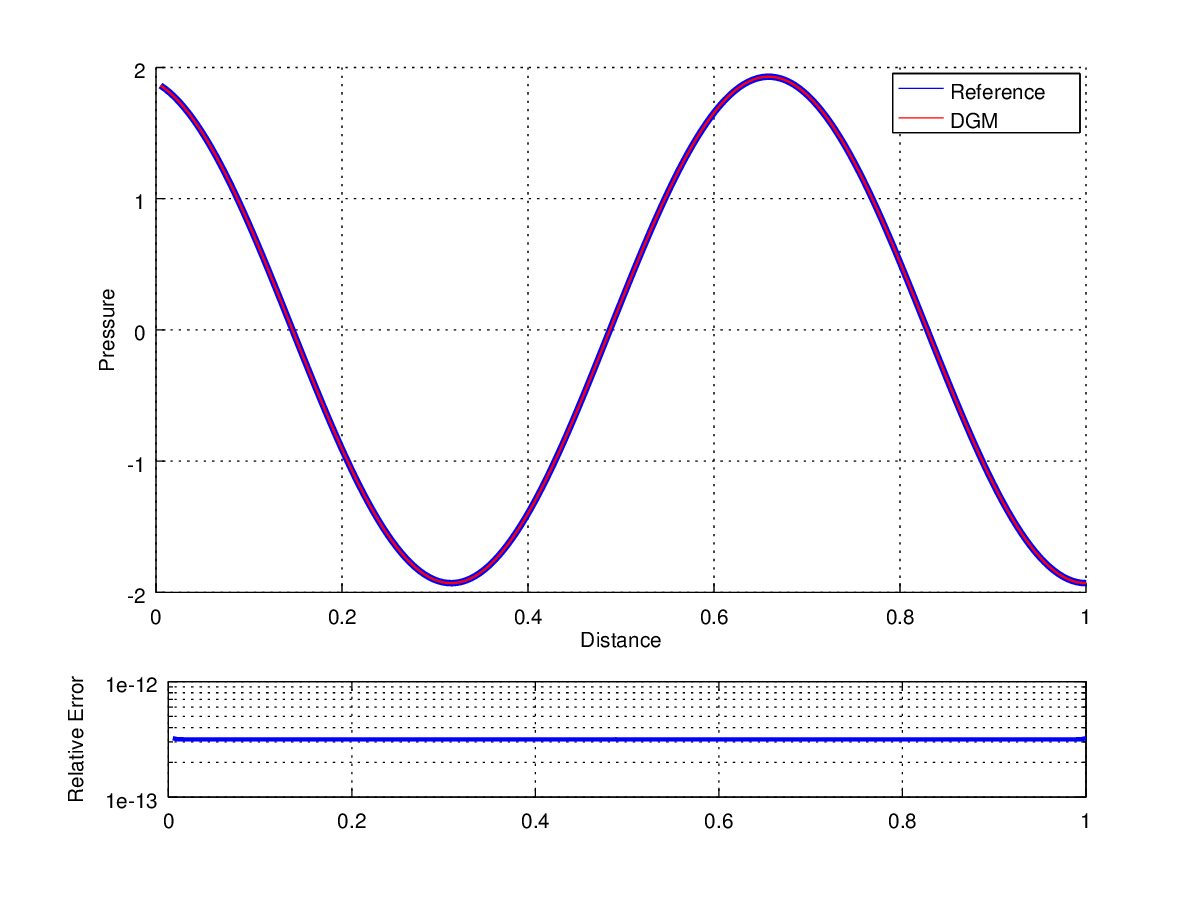
\includegraphics[width=11cm]{part2/figs/comp_hermiteFEM_dgm.png}
    \caption{\label{fig:dgm:simul}En haut : profil de pression dans la cavité par méthode de Galerkin discontinue (en rouge) et
    profil de référence (en bleu). En bas : erreur relative (norme $L_2$ des pressions) pour chaque point.}
\end{figure}

Aucune différence n'est visuellement constatable entre les deux courbes. Qui plus est, l'erreur, à presque $10^{-13}$,
s'approche du bruit numérique.


\part{Méthode de Galerkin Discontinue avec Ondes Planes}
\label{part:dgm}
\newpage\thispagestyle{empty}\null\newpage
\addtocounter{page}{-2}
\setcounter{section}{0}

% TODO intro galerkin

\section{Généralités}

Soit un milieu de propagation où sont valable les équations suivantes :

\begin{eqnarray}
    \left\{\begin{array}{l}
        j\omega\rho v = -\nabla p\\
        p = -\rho c^2 \nabla u
    \end{array}\right.
    & \Leftrightarrow &
    \left\{\begin{array}{l}
        j\omega\rho v = -\nabla p\\
        j\omega p = -\rho c^2 \nabla v
    \end{array}\right.
    \notag\\ & \Leftrightarrow &
    j\omega \begin{Bmatrix}v\\p\end{Bmatrix} + 
    \begin{bmatrix}
        0 & \nicefrac{1}{\rho}\\
        \rho c^2 & 0
    \end{bmatrix}
    \nabla \begin{Bmatrix}v\\p\end{Bmatrix} = 0
    \notag\\ & \Leftrightarrow &
        \left(j\omega + \uul{A}\frac{\partial}{\partial x}\right) \ul{u} = 0 \label{dgm:eq_u}
\end{eqnarray}

L'idée est alors de découpler les équations précédentes en diagonalisant $\uul{A}$, il vient :

\begin{equation*}
    \uul{A} = \uul{P\Lambda Q} \quad,\quad \uul{P} = \uul{Q}^{-1}
\end{equation*}

En posant

\begin{equation}
    \ul{\tilde{u}} = \begin{Bmatrix}\tilde{u}^+\\\tilde{u}^-\end{Bmatrix} = \ul{Q}\ul{u}\label{dgm:utilde}
\end{equation}
l'équation~\eqref{dgm:eq_u} devient :

\begin{equation*}
    j\omega \ul{\tilde{u}} + \uul{\Lambda}\nabla\ul{\tilde{u}} = 0
\end{equation*}

En isolant les valeurs positives et négatives de $\uul{\Lambda}$  (notées $\Lambda^{+,-}$) ainsi que les vecteurs
associés $\ul{P}^{+,-}$ et $\ul{Q}^{+,-}$, il est possible d'écrire :

\begin{equation}
    \left\{\begin{array}{l}
        \tilde{u}^+ = \ul{Q}^+\ul{u}\\
        \tilde{u}^- = \ul{Q}^-\ul{u}
    \end{array}\right. \Leftrightarrow
    \ul{u} = \ul{P}^+\tilde{u} + \ul{P}^-\tilde{u} \label{dgm:sep_u}
\end{equation}


\paragraph{Formulation variationnelle}

En utilisant la formulation variationnelle et une intégration par parties, il vient :

\begin{equation}
    \begin{array}{c}
    \int_\Omega \ul{v}^T\left(j\omega + \uul{F}\nabla\right)\ul{u}\dd\Omega = 0 \quad,\quad \forall\ul{v}\\
    -\left(\int_\Omega j\omega v + \uul{A}^T\nabla\ul{v}\right)^Tu\dd\Omega +
        \int_{\partial\Omega}\ul{v}^T\uul{A}\ul{u}\dd\Gamma = 0 \quad,\quad \forall\ul{v}
    \end{array}
    \label{dgm:post_ipp}
\end{equation}

\paragraph{Nota Bene} Le symbole $\cdot^T$ représente une transposition Hermitienne.

L'objectif est alors de choisir le champ de test $\ul{v}$ permettant d'annuler l'intégrale sur $\Omega$ :

\begin{equation}
    \left(j\omega + \uul{A}^T\nabla\right)\ul{v} = 0 \label{dgm:eq_v}
\end{equation}

De toute l'équation~\eqref{dgm:post_ipp}, il reste alors :

\begin{equation}
    \int_{\partial\Omega}\ul{v}^T\uul{A}\ul{u}\dd\Gamma = 0 \quad,\quad \forall\ul{v}\label{dgm:to_solve}
\end{equation}


\section{Discrétisation des champs}

Le choix des fonctions du champ de test un enjeu prépondérant dans la méthode de Galerkin discontinue.
La suite cherche à discrétiser les champs de tests \textit{via} une base d'ondes planes, comme proposé par Gabard
\textit{et al.}\cite{Gabard15}.

Les expressions des champs discrétisés sont tirées directement de la résolution des équations
différentielles~\eqref{dgm:eq_u} et~\eqref{dgm:eq_v}. Il faut noter que le problème à résoudre pour $\ul{v}$ est l'adjoint
de celui à résoudre pour $\ul{u}$ (la matrice $\uul{A}$ n'étant pas symétrique).

Les solutions recherchés sont donc composées d'une somme d'ondes planes :

\[
    \xi(x) = \xi_+e^{-jkx}+\xi_-e^{+jkx}
\]

La solution pour $\ul{u}$ est donc de la forme :

\begin{equation}
    \ul{u} = \begin{Bmatrix}v\\p\end{Bmatrix} =
    \begin{bmatrix}
        \nicefrac{1}{Z_0} & -\nicefrac{1}{Z_0}\\
        1 & 1
    \end{bmatrix}
    \begin{bmatrix}
        e^{-jkx} & 0\\
        0 & e^{+jkx}
    \end{bmatrix}
    \begin{Bmatrix}
        A\\B
    \end{Bmatrix}
    =
    \underbrace{\begin{bmatrix}
        \nicefrac{e^{-jkx}}{Z_0} & -\nicefrac{e^{+jkx}}{Z_0}\\
        e^{-jkx} & e^{+jkx}
    \end{bmatrix}}_{\uul{U}_u(x)}
    \underbrace{\begin{Bmatrix}
        A\\B
    \end{Bmatrix}}_{\GU}
\end{equation}

Le champ de test $\ul{v}$ est solution du problème adjoint~\eqref{dgm:eq_v}, la solution pour $\ul{v}$ est donc de la forme

\begin{equation}
    \ul{v} =
    \begin{bmatrix}
        Z_0 & -Z_0\\
        1 & 1
    \end{bmatrix}
    \begin{bmatrix}
        e^{-jkx} & 0\\
        0 & e^{+jkx}
    \end{bmatrix}
    \begin{Bmatrix}
        \delta A\\\delta B
    \end{Bmatrix}
    =
    \underbrace{
    \begin{bmatrix}
        Z_0e^{-jkx} & -Z_0e^{+jkx}\\
        e^{-jkx} & e^{+jkx}
    \end{bmatrix}}_{\uul{U}_v(x)}
    \underbrace{\begin{Bmatrix}
        \delta A\\\delta B
    \end{Bmatrix}}_{\GV}
\end{equation}

\section{Problème 1D}

En repartant de~\eqref{dgm:to_solve} et en considérant un problème 1D (voir figure~\ref{fig:FEM:propa_1D}), il vient :

\begin{equation}
    \int_{\partial\Omega}\ul{v}^T\uul{A}\ul{u}\dd\Gamma = 0 \Leftrightarrow
\underbrace{\ul{v}^T(L)\uul{A}\ul{u}(L)}_\mathrm{droite} - \underbrace{\ul{v}^T(0)\uul{A}\ul{u}(0)}_\mathrm{gauche}
\quad,\quad \forall\ul{v}\label{dgm:d_g}
\end{equation}

\subsection{Condition limite à droite}

A droite, la paroi rigide implique :

\begin{eqnarray*}
    v(L) = 0 & \Leftrightarrow &
    \begin{pmatrix}
        1 & 0
    \end{pmatrix}
    \begin{pmatrix}
        v\\p
    \end{pmatrix}
     = 0\\
    & \Leftrightarrow &
    \begin{pmatrix}
        1 & 0
    \end{pmatrix}
    \begin{bmatrix}
        1 & 1\\
        Z_0 & -Z_0
    \end{bmatrix}
    \begin{pmatrix}
        \tilde{u}^+\\\tilde{u}^-
    \end{pmatrix}\\
    & \Leftrightarrow &
    \tilde{u}^+ = -\tilde{u}^- \Leftrightarrow \tilde{u}^+ = R^-\tilde{u}^-
\end{eqnarray*}

En utilisant maintenant~\eqref{dgm:sep_u}, et en réutilisant le résultat précédent :

\begin{eqnarray}
    \ul{u} = \ul{P}^+\tilde{u}^+ + \ul{P}^-\tilde{u}^-
        & \Leftrightarrow & \ul{u} = \ul{P}^+\tilde{u}^+ + \ul{P}^-R^-\tilde{u}^+\notag\\
        & \Leftrightarrow & \ul{u} = \left(\ul{P}^+ + \ul{P}^-R^-\right)\ul{Q}^+u\label{dgm:droite}
\end{eqnarray}

\subsection{Condition limite à gauche}

A gauche, les conditions de continuité impliquent :

\begin{figure}[!ht]
	\centering
	\begin{tikzpicture}
    \draw[thick] (0,-.2) -- (0,0) -- (2.5,0);
    \draw[thick] (0,1.7) -- (0,1.5) -- (2.5,1.5);

    \draw[dashed] (0,0) -- (0,1.5);

    \draw[->] (-2,1) -- ++(1,0) node[midway,above] {$1$};
    \draw[->] (-1,.5) -- ++(-1,0) node[midway,above] {$R$};
    \draw[->] (1,1) -- ++(1,0) node[midway,above] {$\tilde{u}^+$};
    \draw[->] (2,.5) -- ++(-1,0) node[midway,above] {$\tilde{u}^-$};
\end{tikzpicture}


    \caption{\label{fig:interface}Interface à gauche du problème.}
\end{figure}

\begin{equation*}
    \begin{array}{c}
        P\begin{Bmatrix}1\\R\end{Bmatrix} = P\begin{Bmatrix}\tilde{u}^+\\\tilde{u}^-\end{Bmatrix}\\
            \Leftrightarrow \left\{\begin{array}{l}
                    \tilde{u}^+ = 1\\
                    \tilde{u}^- = R = \ul{Q}^-\ul{u}
            \end{array}\right.
    \end{array}
\end{equation*}

En ré-exprimant $u$, il vient :

\begin{equation}
    \ul{u} = \ul{P}^+\tilde{u}^+ + \ul{P}^-\tilde{u}^- \Leftrightarrow \ul{u} = \ul{P}^+ + \ul{P}^-\ul{Q}^-\ul{u}\label{dgm:gauche}
\end{equation}

En remettant~\eqref{dgm:droite} et~\eqref{dgm:gauche} dans~\eqref{dgm:d_g} et en utilisant les expressions discrétisées
des champs, il vient :

\begin{equation}
    \begin{array}{rcl}
        \GV^T\bigg[\uul{U}_v^T(L)\uul{P\Lambda Q}\left(\ul{P}^+ + \ul{P}^-R^-\right)\ul{Q}^+\uul{U}_u(L) & - &
    \uul{U}_u(0)\uul{P\Lambda Q}\ul{P}^-\ul{Q}^-\uul{U}_u(0)\bigg] \GU\\
    & = & \GV^T\uul{U}_v^T(0)\uul{P\Lambda Q}\ul{P}^+ \quad,\quad \forall\GV
    \end{array}
\end{equation}

L'équation précédente étant valable pour tout vecteur $\GV$ il est possible de supprimer ce terme.
La solution pour $\GU$ est alors calculable par simple division matricielle.

\subsection{Simulation}

En 1D, la DGM avec ondes planes présentée ici conduit à une solution exacte. Pour cette simulation, plutôt que l'analyse
de la convergence pour le calcul du coefficient, c'est le tracé du profil de pression qui est réalisé. Le résultat est
présenté en figure~\ref{fig:dgm:simul}.

\begin{figure}[!ht]
    \centering
    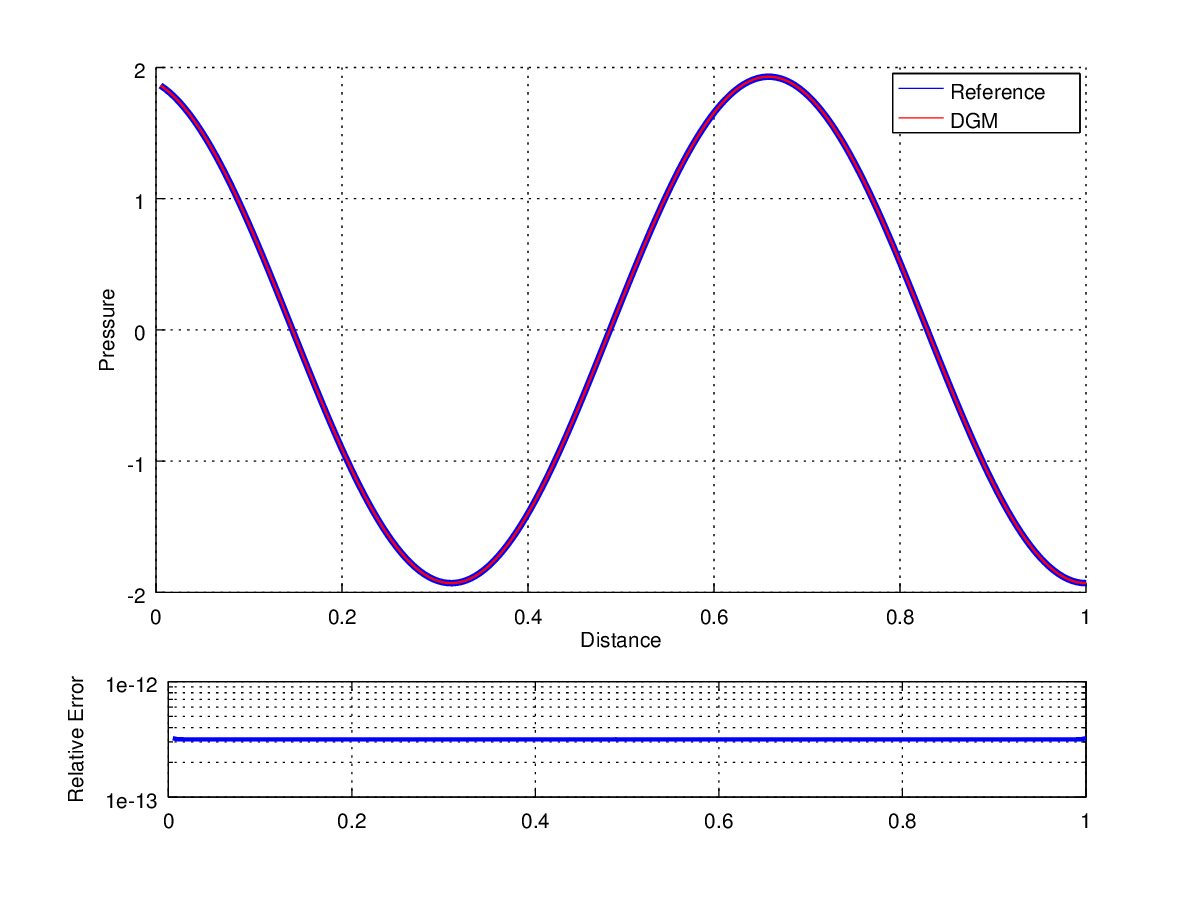
\includegraphics[width=11cm]{part2/figs/comp_hermiteFEM_dgm.png}
    \caption{\label{fig:dgm:simul}En haut : profil de pression dans la cavité par méthode de Galerkin discontinue (en rouge) et
    profil de référence (en bleu). En bas : erreur relative (norme $L_2$ des pressions) pour chaque point.}
\end{figure}

Aucune différence n'est visuellement constatable entre les deux courbes. Qui plus est, l'erreur, à presque $10^{-13}$,
s'approche du bruit numérique.


\part{Couplage -- Caractéristiques et Conditions aux Limites}
\label{part:couplage}
\newpage\thispagestyle{empty}\null\newpage
\addtocounter{page}{-2}
\setcounter{section}{0}
Dans cette section, l'objectif est de proposer une formulation de la condition en limite en $x=0$ du problème présenté
en figure~\ref{fig:rflx:propa_1D} qui n'impose pas de rajouter une ligne au système d'équations de la FEM.

\begin{figure}[!ht]
	\centering
	\begin{tikzpicture}[>=stealth]

	% waveguide
	\draw[thick] (0,.3) -- (0,.5) -- (7,.5) -- (7,2) -- (0,2) -- (0,2.2);
	\foreach \i in {0,...,5}{
		\draw[thick] (7,\i*0.3+0.5) -- ++(.3,.2);
	}
	
	% x axis
	\draw[->] (-.7,0) -- (8,0) node[right] {$x$};
	\draw (0,.1) -- ++(0,-.2) node[below] {$0$};
	\draw (7,.1) -- ++(0,-.2) node[below] {$L$};

	% waves
	% R
	\draw[<-] (-2.5,1) -- ++(1.5,0);
	\draw (-2,1.15) -- ++(0,-.3);
	\draw (-1.9,1.15) -- ++(0,-.3) node[below] {$R$};

	% I
	\draw[->] (-2.5,1.5) -- ++(1.5,0);
	\draw (-2,1.65) -- ++(0,-.3);
	\draw (-1.9,1.65) node[above] {$I$} -- ++(0,-.3);

\end{tikzpicture}


	\caption{\label{fig:rflx:propa_1D}Schéma du problème de propagation dans une cavité acoustique 1D de longueur L.}
\end{figure}

\section{Retour sur les conditions aux limites en FEM}

Pour ce problème et en utilisant le formalisme des éléments finis, le système à résoudre avant l'application de la
condition limite en $x=0$ mais après celle de la condition en $x=L$ est tel que présenté en~\eqref{FEM1D:post_BCL} :

\begin{equation}
\left[- \uul{K} + k^2\uul{M}\right]\GP = \begin{Bmatrix} \nabla p\bigg|_0\\0\\\vdots\\0\end{Bmatrix} \label{rflx:FEM}
\end{equation}


\subsection{Condition en $x=0$ : utilisation des caractérisatiques}

Sous le formalisme de la méthode de Galerkin, il vient :

\begin{equation}
	j\omega\begin{Bmatrix}v\\p\end{Bmatrix} = 
		\underbrace{\begin{bmatrix}0 & \nicefrac{1}{\rho}\\\rho c^2 & 0\end{bmatrix}}_{\uul{F}}
		\begin{Bmatrix}v\\p\end{Bmatrix} \Leftrightarrow j\omega\ul{u} + \uul{P\Lambda Q}\ul{u} = 0
		\label{rflx:begin_dgm}
\end{equation}

Où $\uul{P\Lambda Q}$ est une diagonalisation de $\uul{F}$ telle que :

\[
\uul{P} = \begin{bmatrix}1 & 1\\Z_0 & -Z_0\end{bmatrix} \quad,\quad
\uul{\Lambda} = \begin{bmatrix}c & 0\\0 & -c\end{bmatrix} \quad,\quad
\uul{Q} = \begin{bmatrix}
	\nicefrac{1}{2} & \nicefrac{1}{2Z_0}\\
	\nicefrac{1}{2} & -\nicefrac{1}{2Z_0}\\
\end{bmatrix}
\]

En posant $\ul{\tilde{u}} = \uul{Q}\ul{u}$, le système~\eqref{rflx:begin_dgm} s'écrit simplement $j\omega\ul{\tilde{u}} +
\uul{\Lambda}\ul{\tilde{u}} = 0$ et les conditions aux limites peuvent s'écrire sous la forme $$\uul{C}\ul{u} = \ul{s} \Leftrightarrow
CP\ul{\tilde{u}} = \ul{s}$$

Les conditions de continuité sur $p$ et $v$ permettent d'écrire :

\begin{equation*}
	\left\{
		\begin{array}{l}
			p(0) = 1 + R\\
			v(0) = \frac{1}{Z_0}(1-R)
		\end{array}
	\right.
	\Leftrightarrow
	\begin{bmatrix}
		1 & 0\\
		0 & 1
	\end{bmatrix}
	\begin{Bmatrix}
		v\\
		p
	\end{Bmatrix}_0 = 
	\begin{bmatrix}
		\nicefrac{1}{Z_0} & -\nicefrac{1}{Z_0}\\
		1 & 1
	\end{bmatrix}
	\begin{Bmatrix}
		1\\
		R
	\end{Bmatrix}
\end{equation*}

Soit, en insérant le produit $\uul{PQ}$ :

\begin{eqnarray*}
	\uul{P}
	\begin{Bmatrix}
		\tilde{u}^+\\
		\tilde{u}^-
	\end{Bmatrix}_0 & = &
	\begin{bmatrix}
		\nicefrac{1}{Z_0} & -\nicefrac{1}{Z_0}\\
		1 & 1
	\end{bmatrix}
	\begin{Bmatrix}
		1\\
		R
	\end{Bmatrix}\\
	\Leftrightarrow
	\begin{Bmatrix}
		\tilde{u}^+\\
		\tilde{u}^-
	\end{Bmatrix}_0 & = &
	\begin{bmatrix}
		\nicefrac{1}{2} & \nicefrac{1}{2Z_0}\\
		\nicefrac{1}{2} & -\nicefrac{1}{2Z_0}\\
	\end{bmatrix}
	\begin{bmatrix}
		\nicefrac{1}{Z_0} & -\nicefrac{1}{Z_0}\\
		1 & 1
	\end{bmatrix}
	\begin{Bmatrix}
		1\\
		R
	\end{Bmatrix}\\
	\Leftrightarrow
	\begin{Bmatrix}
		\tilde{u}^+\\
		\tilde{u}^-
	\end{Bmatrix}_0 & = &
	\begin{bmatrix}
		\nicefrac{1}{Z_0} & 0\\
		0 & -\nicefrac{1}{Z_0}
	\end{bmatrix}
	\begin{Bmatrix}
		1\\
		R
	\end{Bmatrix}\\
\end{eqnarray*}

Les relations d'intérêt sont donc :

\begin{equation}
	\left\{
		\begin{array}{l}
			\tilde{u}^+_0 = \nicefrac{1}{Z_0}\\
			\tilde{u}^-_0 = -\nicefrac{R}{Z_0}\\
		\end{array}
	\right. \label{rflx:useful_rels}
\end{equation}


\subsection{Interpolation des caractéristiques}

Le système~\eqref{rflx:useful_rels} est écrit en fonction des caractéristiques $\tilde{u}^\pm$, et il conviendrait de
l'exprimer en utilisant les fonctions de forme $(\phi_1, \ldots, \phi_N)$ introduites par la méthode des éléments finis.

\paragraph{Nota Bene} Dans la suite de la démonstration, ne sont utilisés que des éléments linéaires pour alléger les
calculs. Le concept est exactement le même pour des éléments quadratiques.

\medskip

Ainsi, il vient\footnote{La seconde étant déduite de la première \textit{via} l'équation d'Euler.} :

\begin{equation*}
	p(0) = \phi_1(0)\GP_1 + \phi_2(0)\GP_2 \quad\mathrm{et}\quad v(0) = \frac{-1}{j\omega\rho}\left(\phi'_1(0)\GP_1 +
		\phi'_2(0)\GP_2\right)
\end{equation*}

Soit :

\begin{equation*}
	\begin{Bmatrix}v\\p\end{Bmatrix}_0 = \underbrace{\begin{bmatrix}
		-\frac{\phi'_1(0)}{j\omega\rho} & -\frac{\phi'_2(0)}{j\omega\rho}\\
		\phi_1(0) & \phi_2(0)
\end{bmatrix}}_{W}
	\begin{Bmatrix}
		\GP_1\\\GP_2
	\end{Bmatrix}
\end{equation*}

En reprenant enfin la définition des $\tilde{u}^{+,-}$, il vient :

\begin{equation*}
\begin{Bmatrix}
	\tilde{u}^+\\\tilde{u}^-
\end{Bmatrix}_0 = Q\begin{Bmatrix}
	v\\p
\end{Bmatrix}_0 = QW\begin{Bmatrix}\GP_1\\\GP_2\end{Bmatrix}
\end{equation*}

En développant il vient notamment :

\begin{equation}
	\tilde{u}^-_0 = -\frac{1}{2Z_0}\left[\left(\phi_1(0) + \frac{\phi'_1(0)}{jk}\right)\GP_1 + \left(\phi_2(0) + \frac{\phi'_2(0)}{jk}\right)\GP_2 \right]\label{rflx:utildem}
\end{equation}

Finalement, la quantité d'intérêt est $\nabla p\big|_0$, accessible depuis $v(0)$ via l'équation d'Euler.

\pagebreak

D'après la définition des $\tilde{u}^\pm$ :


\begin{equation*}
\begin{Bmatrix}
	v\\p
\end{Bmatrix}_0
= W\begin{Bmatrix}
	\tilde{u}^+\\\tilde{u}^-
\end{Bmatrix}_0 \Leftrightarrow
v = \tilde{u}^+_0 + \tilde{u}^-_0
%\label{rflx:def_v}
\end{equation*}

En prenant $\tilde{u}^+_0$ tel que défini en~\eqref{rflx:useful_rels} et $\tilde{u}^-_0$ comme indiqué
en~\eqref{rflx:utildem} il vient :

\begin{equation*}
	\begin{array}{c}
	v(0) = \frac{1}{Z_0} -\frac{1}{2Z_0}\left[\left(\phi_1(0) + \frac{\phi'_1(0)}{jk}\right)\GP_1 + \left(\phi_2(0) + \frac{\phi'_2(0)}{jk}\right)\GP_2 \right]\\
	\Leftrightarrow\quad \nabla p\bigg|_0 = - jk -\frac{jk}{2}\left[\left(\phi_1(0) + \frac{\phi'_1(0)}{jk}\right)\GP_1 + \left(\phi_2(0) + \frac{\phi'_2(0)}{jk}\right)\GP_2 \right]
	\end{array}
\end{equation*}


En retranscrivant cette condition dans le système~\eqref{rflx:FEM}, il est alors possible de résoudre le problème sans
faire apparaître $R$. Cette quantité servant (dans le cadre de ce document) de référence pour les comparaisons, il est
bon de remarquer que $R$ peut facilement être retrouvé en utilisant~\eqref{rflx:utildem} et la seconde équation
de~\eqref{rflx:useful_rels}.

\section{Influence sur la convergence}

La simulation présentée ici utilise des éléments quadratiques. En effet, cette méthode demandant de dériver les
fonctions de forme, elle ne pourrait qu'être désastreuse avec des fonctions d'interpolation linéaires.

En figure~\ref{fig:conv_DGMlike_quad} est présentée l'évolution de l'erreur relative commise par l'approximation en
fonction du nombre d'éléments.

La courbe noire représente l'erreur commise par la méthode classique, avec l'ajout du $R$ aux inconnues. La courbe rouge
présente l'erreur que commet la méthode basée sur les caractéristiques pour l'écriture des conditions aux limites. Il
est à noter que l'utilisation de la formulation par caractéristiques semble donner de moins bons résultats : en effet,
le fait de devoir dériver les fonctions de forme fait qu'un ordre de convergence est perdu.

\begin{figure}[!ht]
	\centering
	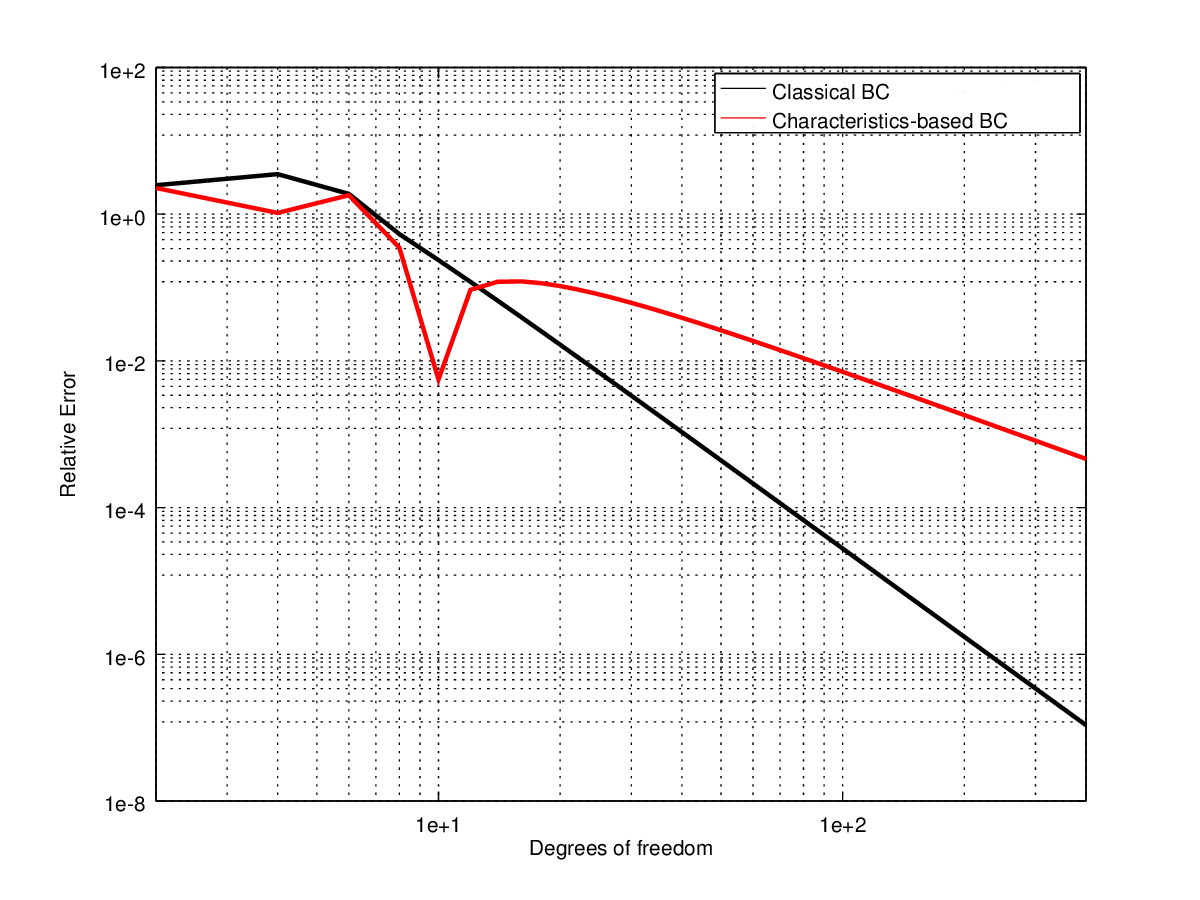
\includegraphics[width=10cm]{part3/figs/convergence.png}
	\caption{\label{fig:conv_DGMlike_quad}Erreur commise par les deux méthodes (ajout du coefficient de réflexion aux
	inconnues et caractéristiques) en fonction du nombre d'éléments utilisé. L'étude est réalisée uniquement pour des
	éléments quadratiques. Il faut noter que l'utilisation des caractériques donne de moins bons résultats dans ce cas.}
\end{figure}


\part{Amélioration de la convergence}
\label{part:convergence}
\newpage\thispagestyle{empty}\null\newpage
\addtocounter{page}{-2}
\setcounter{section}{0}
Comme dit à la fin de la partie~\ref{part:couplage}, la formulation des conditions limites au moyen des
caractéristiques conduit à la dérivation des fonctions de forme classiques. Ce point est clairement un désavantage pour
cette méthode car elle force la perte d'un ordre de convergence.

Dans cette partie, un nouveau jeu de fonctions d'interpolation est proposé dans le but de pallier ce problème. Afin
d'évaluer la pertinence de la proposition, la comparaison est réalisée entre des éléments quadratiques et la base
proposée pour une formulation par caractéristiques d'une part et sans d'autre part.

\section{Une nouvelle interpolation : les splines d'Hermite}

Un moyen d'éviter la perte d'un ordre de convergence à l'utilisation de la méthode par caractéristiques serait
d'utiliser un ensemble de fonctions d'interpolation permettant l'accès direct à la dérivée de la quantité.

L'interpolation par splines d'Hermite utilise 4 «degrés de libertés» répartis sur les deux extrémité du segment à
interpoler : 2 pour le champ lui-même et 2 pour sa dérivée.

Le champ interpolé pour un segment $e$ d'extrémités $1$ et $2$ est défini tel que :

\begin{equation*}
	p_e(x) = \underbrace{\left[\H{00}(x)\big|\H{10}(x)\big|\H{01}(x)\big|\H{11}(x)\right]}_{H}\begin{Bmatrix}p_1\\p'_1\\p_2\\p'_2\end{Bmatrix}
\end{equation*}

Il en va de même pour $v_e$ en remplaçant simplement les valeurs dans le vecteur colonne et $p'_e$ ou $v'_e$ en
reprenant le vecteur colonne de leur homologue non dérivé et en dérivant les fonctions d'interpolation\footnote{Le
vecteur est alors noté $H'$.}.

Les expressions desdites fonctions sont explicitées en annexe~\ref{app:splines}.

En suivant une méthode tout à fait analogue à celle développée pour le calcul des matrices élémentaires en partie~\ref{part:fem}, il vient :

\begin{equation*}
	\uul{M_e} = H^TH \quad,\quad \uul{K_e} = H'^TH'
\end{equation*}

\subsection{Formulation classique}

La formulation classique revient, une fois de plus, à considérer le coefficient de réflexion $R$ comme une inconnue.

Cette méthode ayant déjà été détaillée en partie~\ref{part:fem}, elle ne sera pas ré-expliquée ici. Le fait de
considérer une interpolation par spines d'Hermite change en effet l'implémentation mais pas les expresions
fonctionnelles.

\subsection{Méthode des caractéristiques}

De manière tout à fait semblable à ce qui a été mis en place en partie~\ref{part:couplage}, il vient :

\begin{eqnarray*}
	p_e(0) & = & \underbrace{\left[\H{00}(0)\big|\H{10}(0)\big|\H{01}(0)\big|\H{11}(0)\right]}_{H}\begin{Bmatrix}\GP_1\\\GP_2\\\GP_3\\\GP_4\end{Bmatrix}\\
	v_e(0) = -\frac{1}{j\omega\rho}\nabla p\bigg|_0& = & -\frac{1}{j\omega\rho}\underbrace{\left[\Hp{00}(0)\big|\Hp{10}(0)\big|\Hp{01}(0)\big|\Hp{11}(0)\right]}_{H}\begin{Bmatrix}\GP_1\\\GP_2\\\GP_3\\\GP_4\end{Bmatrix}
\end{eqnarray*}

Le seul point important étant ici de bien garder en tête que le vecteur $\GP$ contient les valeurs du champ de pression
aux points voulues entrelacées avec les valeurs de la dérivée de ce même champ.

En évaluant les polynômes et leurs dérivées en $0$, et avec $\tilde{\ul{u}}_0 = \uul{Q}\ul{u}_0$ :

\begin{eqnarray*}
\begin{Bmatrix}\tilde{u}^+\\\tilde{u}^-\end{Bmatrix}_0 & = &
\begin{bmatrix}
	\nicefrac{1}{2} & \nicefrac{1}{2Z_0}\\
	\nicefrac{1}{2} & -\nicefrac{1}{2Z_0}\\
\end{bmatrix}
\begin{bmatrix}
	0 & -\frac{1}{j\omega\rho} & 0 & 0\\
	1 & 0 & 0 & 0\\
\end{bmatrix}
\begin{Bmatrix}\GP_1\\\GP_2\\\GP_3\\\GP_4\end{Bmatrix}\\
& = & \begin{bmatrix}
	\nicefrac{1}{2Z_0} & -\frac{1}{2j\omega\rho} & 0 & 0\\
	-\nicefrac{1}{2Z_0} & -\frac{1}{2j\omega\rho} & 0 & 0\\
\end{bmatrix}
\begin{Bmatrix}\GP_1\\\GP_2\\\GP_3\\\GP_4\end{Bmatrix}\\
\end{eqnarray*}

Sachant que~\eqref{rflx:useful_rels} et~\eqref{rflx:def_v} sont toujours valables, il vient :

\begin{eqnarray*}
v(0) & = & \tilde{u}^+_0+\tilde{u}^-_0 = \frac{1}{Z_0} - \frac{1}{2Z_0}\GP_1 - \frac{1}{j\omega\rho}\GP_2\\
\nabla p\bigg|_0 & = & -j\omega\rho v(0) = -jk + \frac{jk}{2}\GP_1 + \frac{1}{2}\GP_2
\end{eqnarray*}

Cette expression est alors à remplacer dans le second membre de~\eqref{FEM1D:post_BCL} et la résolution peut se faire
par simple division.

\section{Etude de convergence}


\clearpage

\section*{Conclusion}

La présentation et l'introduction aux méthodes considérées, qui ne devait initialement pas prendre beaucoup de temps, a
en fait été le point principal de ce projet. Les méthodes étant nouvelles il aura fallu les prendre en main et apprendre
à s'en servir, ce qui n'était pas forcément aisé.

Le second temps, à savoir le couplage entre ces deux méthodes, s'est avéré au moins aussi instructif que le premier et a
conduit à une réflexion autour des effets liés au couplage numérique. Plus qu'écrire des équations, cela aura demandé
d'asseoir les connaissances sur les méthodes en jeu et de prendre en compte des petits détails qu'il est souvent
agréable de passer sous silence.

Cette conclusion marque ainsi la fin d'un projet extrèmement instructif et intéressant mais aussi (et surtout) le début d'une
suite. En effet, beaucoup de pistes sont envisageables pour poursuivre la quête du couplage idéal  : aucune vraie
expérience n'a été menée dans ce projet qui se contente de poser les bases du concept. De plus, tout les cas
présentés ici sont des cas 1D, le passage en 2D, s'il est avant tout technique, demandera très certainement un travail
supplémentaire pour écrire les équations du couplage. Une analyse de la rapidité d'une méthode mixte aurait aussi un
intérêt non négligeable et passera probablement par la mise en place de tests objectifs ; suivant les résultats,
certains pans des scripts devront peut être être réécrits pour accélérer le tout. Pour finir sur une touche plus
informatique, l'analyse des maillages aura aussi une importance capitale pour choisir automatiquement la méthode la
plus adaptée à chaque partie du maillage.

Au fur et à mesure des années, je tend à me rapprocher du monde des numériciens et ce projet m'a beaucoup plus pour ça.
Les discussions avec Olivier Dazel concernant les mathématiques et l'analyse numérique m'ont fait entrevoir qu'il y
avait, derrière une première couche un peu difficile d'accès, un monde d'ingéniosité pour contourner de manière élégante
les limites de la science. Ce projet a définitivement eu l'avantage de me forcer à creuser plus avant des points que je
pensais commencer à maîtriser : la remise en question est toujours un bon moteur.


% previous style : alpha
\nocite{*}
\bibliographystyle{alpha}
\bibliography{biblio}

\appendix
\part*{Annexes}
\newpage\thispagestyle{empty}\null\newpage
\addtocounter{page}{-2}

\chapter{Splines d'Hermite}
\label{app:splines}

Les fonctions utilisées pour l'interpolation par spline d'Hermite sont définies telles que\cite{WPSplines} :

\begin{equation*}
\left\{
\begin{array}{l}
	h_{00}(t) = 2t^3-3t^2+1 \\
	h_{10}(t) = t^3-2t^2+t \\
	h_{01}(t) = -2t^3+3t^2 \\
	h_{11}(t) = t^3-t^2 \\
\end{array}
\right.
\end{equation*}


L'approximation sur le segment $(0,h)$ demande d'utiliser une version adaptée des polynômes :

\begin{equation*}
\left\{
\begin{array}{l}
	\H{00}(t) = 2\left(\nicefrac{t}{h}\right)^3-3\left(\nicefrac{t}{h}\right)^2+1 \\
	\H{10}(t) = \left(\nicefrac{t}{h}\right)^3-2\left(\nicefrac{t}{h}\right)^2+\left(\nicefrac{t}{h}\right) \\
	\H{01}(t) = -2\left(\nicefrac{t}{h}\right)^3+3\left(\nicefrac{t}{h}\right)^2 \\
	\H{11}(t) = \left(\nicefrac{t}{h}\right)^3-\left(\nicefrac{t}{h}\right)^2 \\
\end{array}
\right.
\end{equation*}




\end{document}
